In this section,
the performance of the proposed \TAIL{} is evaluated in comparison with baselines.
To support the evaluation,
different simulated tasks with varying difficulty levels ranging from simple to complex ones were utilized.
The details of these tasks are described in the next subsection.

\subsection{Experimental Settings}
\subsubsection{Simulated Tasks}


In order to examine the effectiveness of the proposed method,
six simulated tasks with varying difficulties were considered:
Pendulum \cite{Env_OpenAIGym},
CartPole \cite{Env_OpenAIGym, Env_CartPole},
WindowOpen \cite{Env_MetaWorld},
WindowClose \cite{Env_MetaWorld},
Door \cite{Env_Adroit},
and Hammer \cite{Env_Adroit}.
The task difficulty is varied along two axes;
the size of the state space and the size of the action space.
The detailed descriptions and visualizations of these tasks are shown in Table \ref{tab:Tasks} and Figure \ref{fig:Tasks}.
From such tasks,
three experiments were conducted,
each of which included two different tasks---a source task and a target task.
The detailed descriptions of these experiments are shown in Table \ref{tab:Experiments}.

\begin{landscape}

  \begin{table}[H]
    \caption{Description of six simulated tasks used in the experiment.\label{tab:Tasks}}

    \begin{tabular}{lcccp{5.5cm}}
      \toprule
      \textbf{Task}                               & \textbf{Size of State Space} & \textbf{Size of Action Space}                                              & \textbf{Difficulty Level} & \textbf{Description} \\
      \midrule
      Pendulum \cite{Env_OpenAIGym}               & 3 (continuous)               & 1 (continuous)
                                                  & Easy                         & Swinging up a pendulum.                                                                                                       \\
      CartPole \cite{Env_OpenAIGym, Env_CartPole} & 4 (continuous)               & 1 (continuous)
                                                  & Easy                         & Preventing the pendulum from falling over by applying a force to the cart.                                                    \\
      WindowOpen \cite{Env_MetaWorld}             & 39 (continuous)              & 4 (continuous)
                                                  & Medium                       & Opening a window.                                                                                                             \\
      WindowClose \cite{Env_MetaWorld}            & 39 (continuous)              & 4 (continuous)
                                                  & Medium                       & Closing a window.                                                                                                             \\
      Door \cite{Env_Adroit}                      & 39 (continuous)              & 28 (continuous)
                                                  & Hard                         & A 24-DoF hand attempts to undo the latch and swing the door open.                                                             \\
      Hammer \cite{Env_Adroit}                    & 46 (continuous)              & 26 (continuous)
                                                  & Hard                         & A 24-DoF hand attempts to use a hammer to drive the nail into the board.                                                      \\
      \bottomrule
    \end{tabular}
  \end{table}
\end{landscape}


\begin{figure}[H]
  \centering
  \begin{subfigure}[b]{0.2\textwidth}
    \centering
    \frame{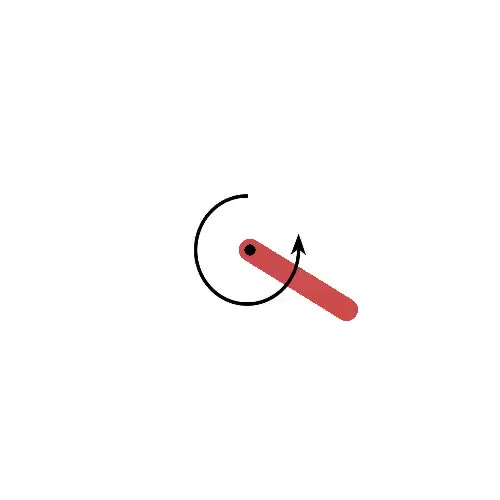
\includegraphics[width=\textwidth]{\FigsDir/Pendulum.jpg}}
    \caption{Pendulum}
  \end{subfigure}
  %
  \hfill
  %
  \begin{subfigure}[b]{0.2\textwidth}
    \centering
    \frame{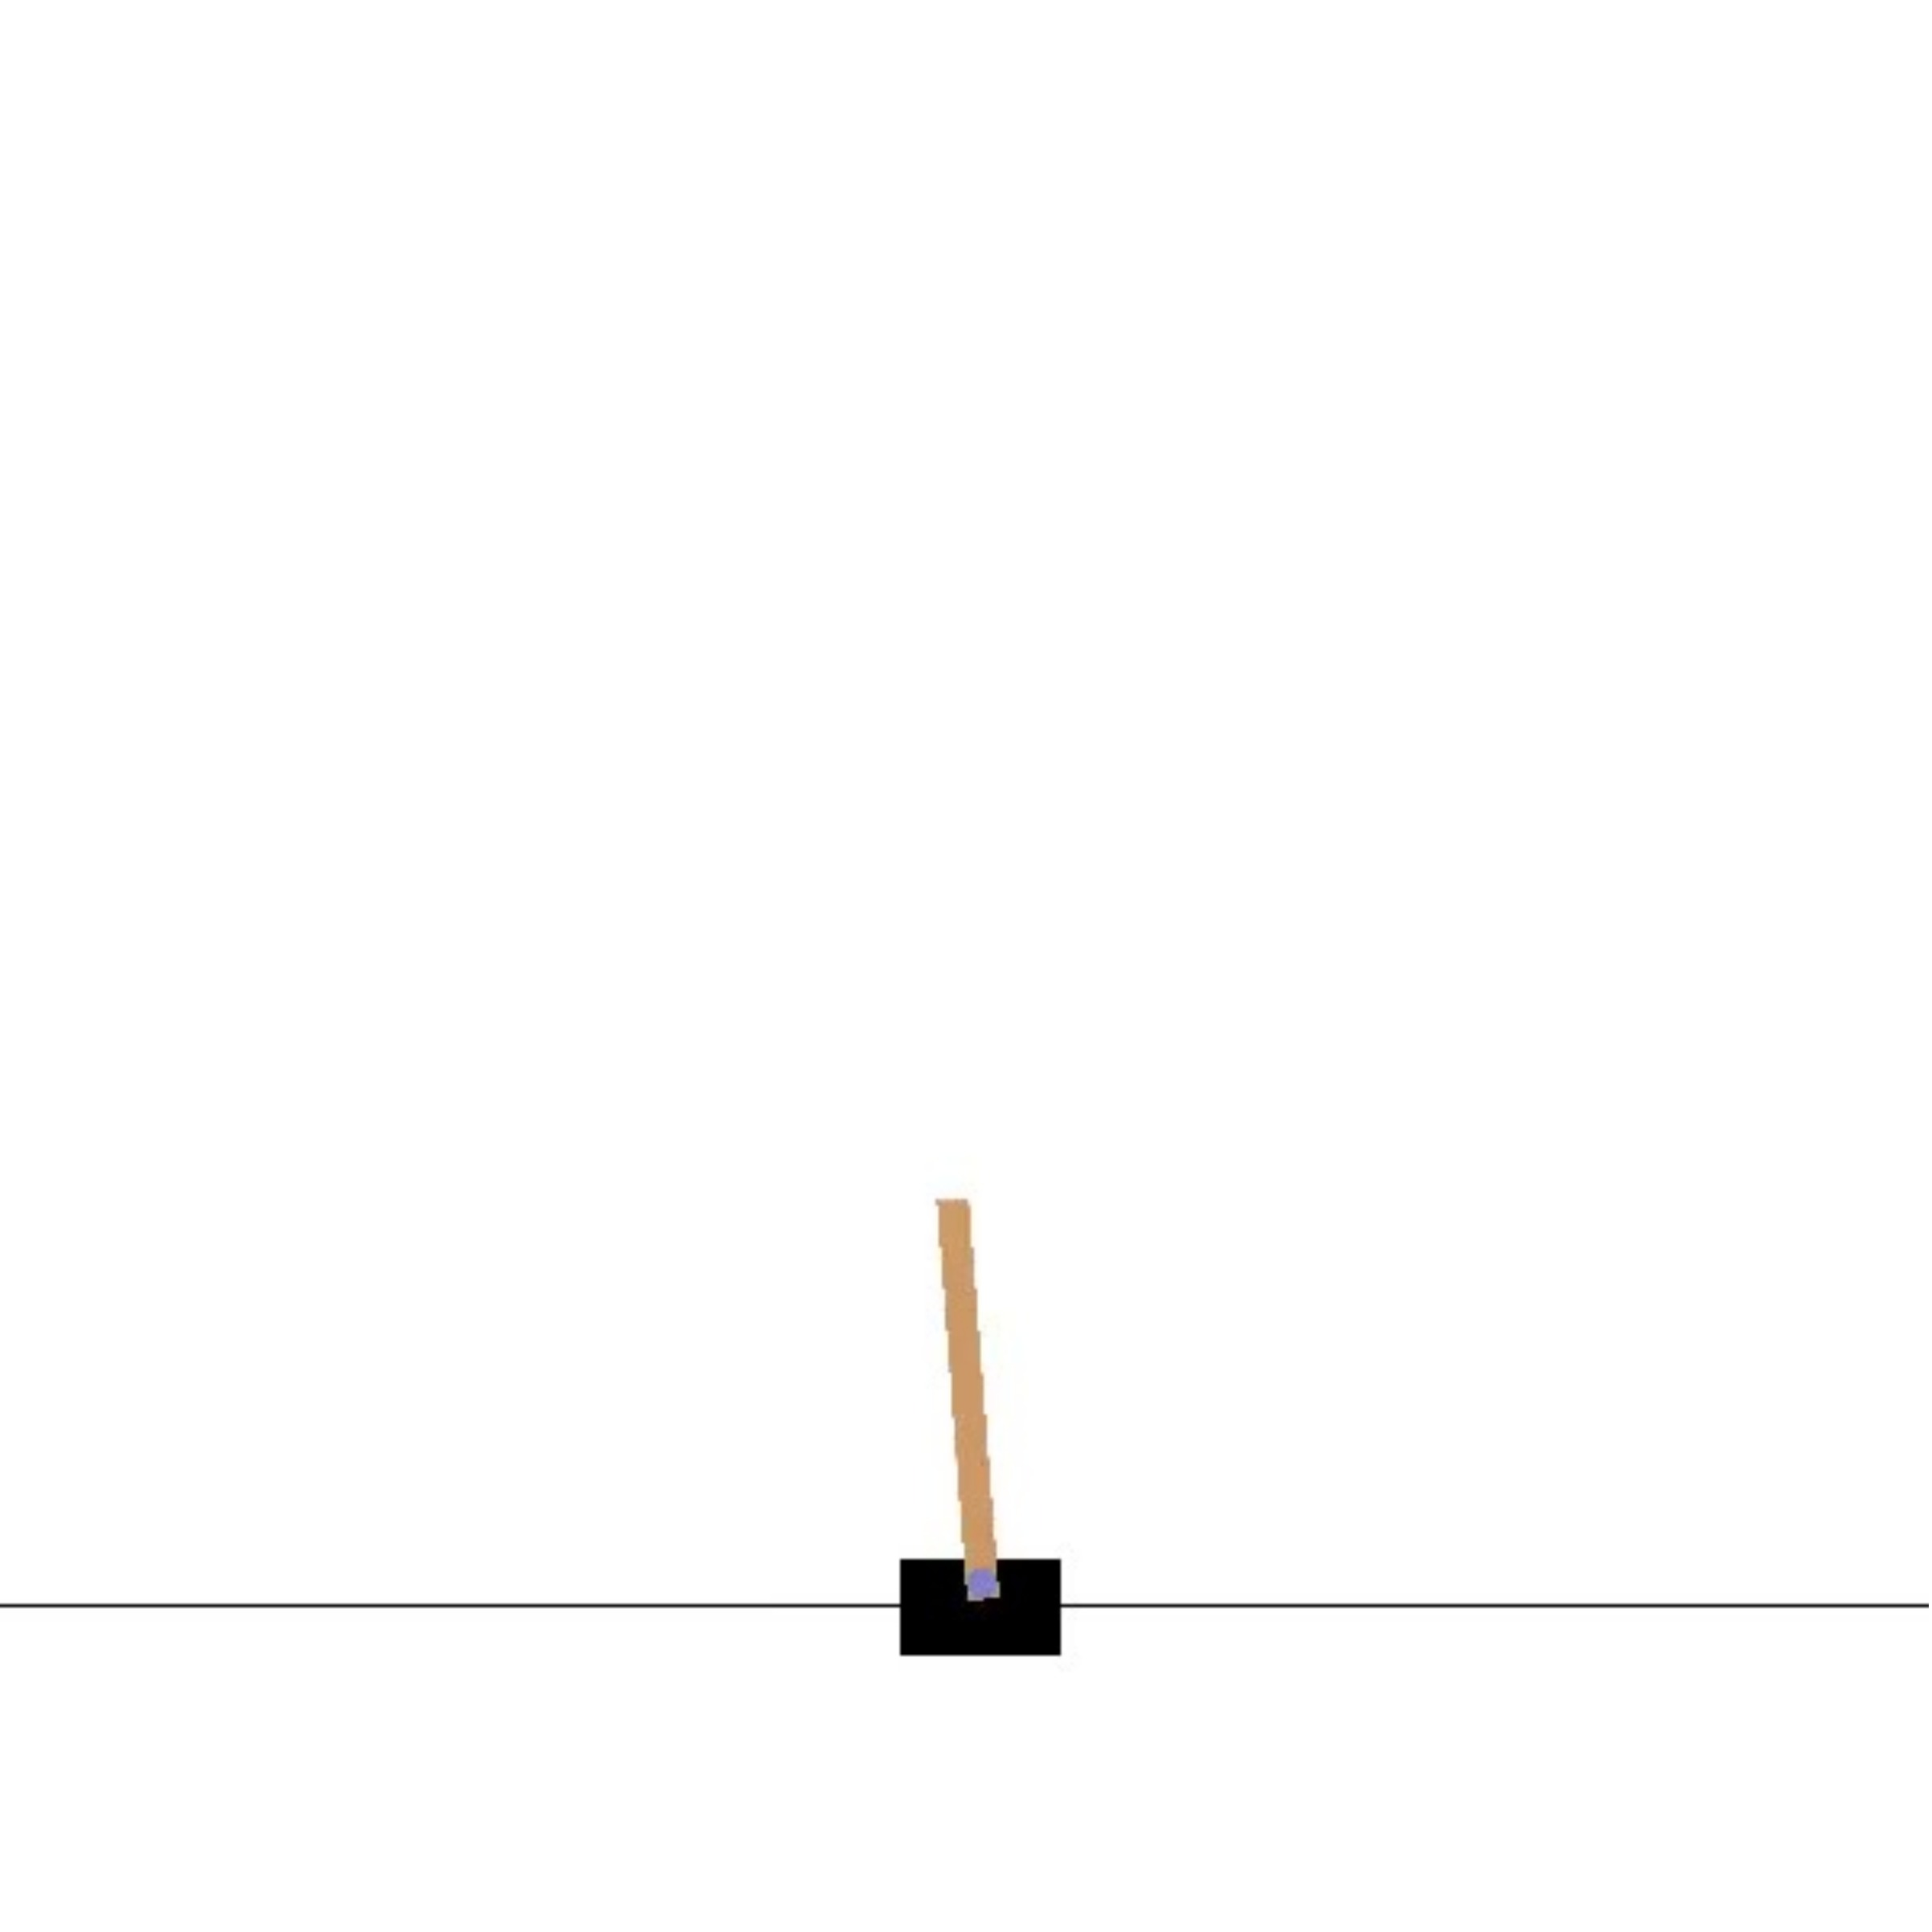
\includegraphics[width=\textwidth]{\FigsDir/CartPole.jpg}}
    \caption{CartPole}
  \end{subfigure}
  %
  \hfill
  %
  \begin{subfigure}[b]{0.25\textwidth}
    \centering
    \frame{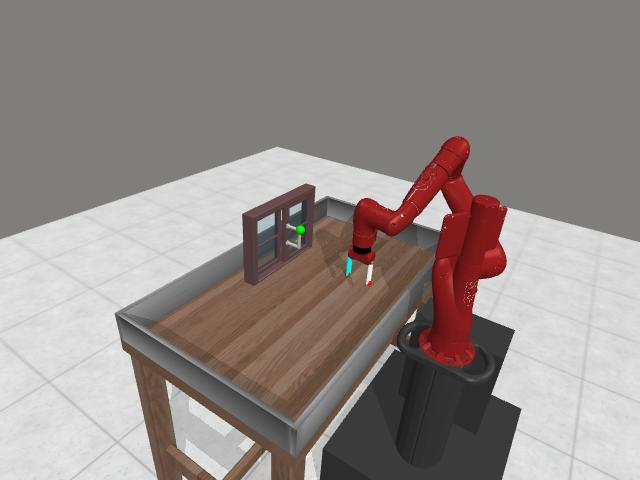
\includegraphics[width=\textwidth]{\FigsDir/WindowOpen.jpg}}
    \caption{WindowOpen}
  \end{subfigure}
  %
  \hfill
  %
  \begin{subfigure}[b]{0.25\textwidth}
    \centering
    \frame{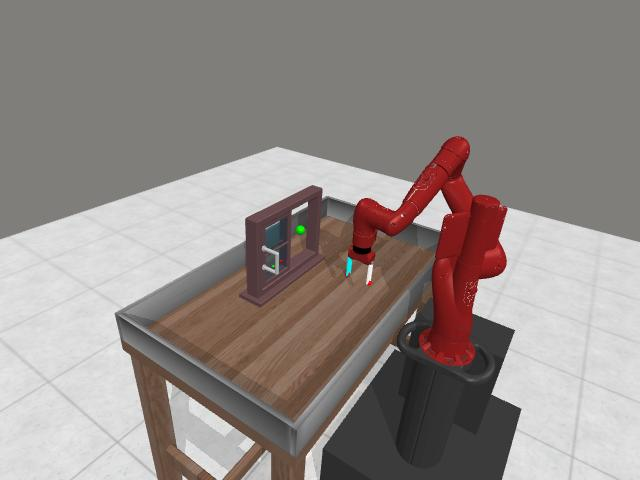
\includegraphics[width=\linewidth]{\FigsDir/WindowClose.jpg}}
    \caption{WindowClose}
  \end{subfigure}\\
  %
  \par\bigskip
  %
  \begin{subfigure}[b]{0.2\textwidth}
    \centering
    \frame{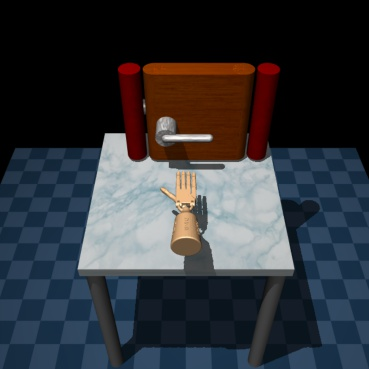
\includegraphics[width=\linewidth]{\FigsDir/Door.jpg}}
    \caption{Door}
  \end{subfigure}
  %
  % \hfill
  %
  \hspace{4em}
  \begin{subfigure}[b]{0.2\textwidth}
    \centering
    \frame{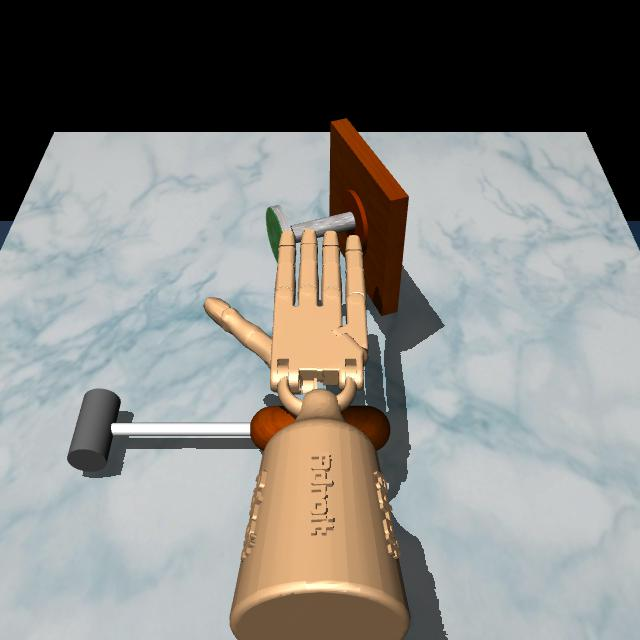
\includegraphics[width=\linewidth]{\FigsDir/Hammer.jpg}}
    \caption{Hammer}
  \end{subfigure}
  %
  \caption{Visual rendering of five simulated tasks used in the experiment.\label{fig:Tasks}}
\end{figure}
\unskip

\begin{landscape}
  \begin{table}[H]
    \centering
    \caption{Description of three experiments conducted to evaluate the performance of the proposed method.\label{tab:Experiments}}

    \begin{tabular}{lcccp{5.5cm}}
      \toprule
      \textbf{Experiment}     & \textbf{Source Task} & \textbf{Target Task}                                                                               & \textbf{Difficulty Level} & \textbf{Description} \\
      \midrule
      Pendulum--CartPole      & Pendulum             & CartPole
                              & Easy                 & A simple experiment in which both source and target tasks have small state and action spaces.                                                         \\
      WindowOpen--WindowClose & WindowOpen           & WindowClose
                              & Medium               & Both source and target tasks have a large state space but small action space.                                                                         \\
      Door--Hammer            & Door                 & Human
                              & Hard                 & A challenging experiment in which both source and target tasks have large state and action spaces.                                                    \\
      \bottomrule
    \end{tabular}
  \end{table}
\end{landscape}

In order to train and adapt the proposed \TAIL{} agent,
expert demonstrations for both source and target tasks must be provided.
In this experiment,
the proximal policy optimization (PPO) method was chosen to be trained on each task in order to create an expert RL agent.
The reason behind this decision was that PPO was recently showing the best result for many complex tasks.
After that,
the demonstrations were collected by executing the trained PPO expert agent in the simulated task.
For the source task, 30 demonstrations were collected to provide sufficient data for training the proposed agent \cite{IL_Model_GAIL}.
In the adaptation process, the proposed agent already learned the knowledge of the source task, thus, a smaller number of demonstrations for the target task is required.
Therefore, only 15 demonstrations were collected for the target task.


%==================================================
\subsubsection{Baselines}


To evaluate the performance of the proposed agent,
two baselines were considered.
\begin{description}
  \item[PPO + Fine-tuning]
        The agent is trained on the source task using Proximal Policy Optimization (PPO) \cite{Baseline_PPO}, which is a policy optimization method.
        Then, fine-tuning is applied to adapt the trained agent to the target task.
        Fine-tuning is a common transfer learning technique that simply re-trains the agent on a new target task.

  \item[NFQI + TA-TL]
        NFQI + TA-TL is a policy adaptation method, where first it utilizes  Neural Fitted Q-iteration (NFQI) \cite{Baseline_NFQI} to find an optimal policy on a source task,
        then that policy is transferred to a new target task.
        NFQI is a Q-learning method that tries to estimate the Q-function using a deep feed-forward network.
\end{description}

In order to provide a fair comparison,
each baseline was evaluated for 100 trials.
The success rate and average cumulative reward were used as performance metrics.
The success rate indicates the percentage of trials in which the baseline can successfully complete a task.
The average cumulative reward measures how well the baseline performed in a trial.

\subsection{Results}

The result is tabulated in Table \ref{ch:TAIL:tab:Result_SuccessRate_After_Target}.
The behavior of those agents when performing target tasks is visualized in Figure \ref{fig:Result_After_Target}.
It can be seen that the proposed \TAIL{} and baselines provide comparably similar behaviors in order to solve target tasks.
This result indicated that the proposed agent successfully adapted and transferred the agent's knowledge to the new target task.
Moreover, it can be observed from Table \ref{ch:TAIL:tab:Result_SuccessRate_After_Target} that \TAIL{} outperformed other baselines.
In addition, it performed highly well and consistently on the complex WindowClose and Hammer tasks.
Applying fine tuning to the PPO agent also provided a consistent performance across all three tasks.
At the same time, applying TA-TL to the NFQI agent was not able to produce a high success rate due to the high complexity of the WindowClose and Hammer tasks.


The results demonstrated that the proposed agent not only outperformed baselines in terms of success rate on all target tasks, but notably produced a consistently high performance, even on the most difficult task.
This proved the potential of the proposed agent and adversarial learning in order to tackle the task adaptation problem in imitation learning.

\begin{table}[H]
  \footnotesize
  \caption{The performance of the proposed agent on target tasks after adaptation. \label{ch:TAIL:tab:Result_SuccessRate_After_Target}}

  \centering
  \setlength{\tabcolsep}{.7mm}{\begin{tabular}{llccc}
      \toprule
       &                                       & \textbf{CartPole} & \textbf{WindowClose} & \textbf{Hammer}       \\
      \midrule
      \multirow{4}{*}{Success rate}
       & \TAIL{}                               & 100\%             & 85\%                 & 80\%                  \\
       & PPO \cite{Baseline_PPO} + Fine-tuning & 100\%             & 82\%                 & 76\%                  \\
       & NFQI + TA-TL \cite{Baseline_TATL}     & 100\%             & 77\%                 & 70\%                  \\
      \midrule
      \multirow{4}{*}{Average cumulative reward}
       & \TAIL{}                               & $500.00 \pm 0.0$  & $2473.10 \pm 619.13$ & $3351.69 \pm 1957.30$ \\
       & PPO \cite{Baseline_PPO} + Fine-tuning & $500.00 \pm 0.0$  & $2402.65 \pm 638.54$ & $3165.05 \pm 1134.02$ \\
       & NFQI + TA-TL \cite{Baseline_TATL}     & $500.00 \pm 0.0$  & $1457.53 \pm 621.37$ & $2840.35 \pm 1036.76$ \\
      \bottomrule
    \end{tabular}}
\end{table}



\begin{landscape}
  \begin{figure}[H]
    \centering
    %
    \begin{subfigure}[b]{\linewidth}
      \centering
      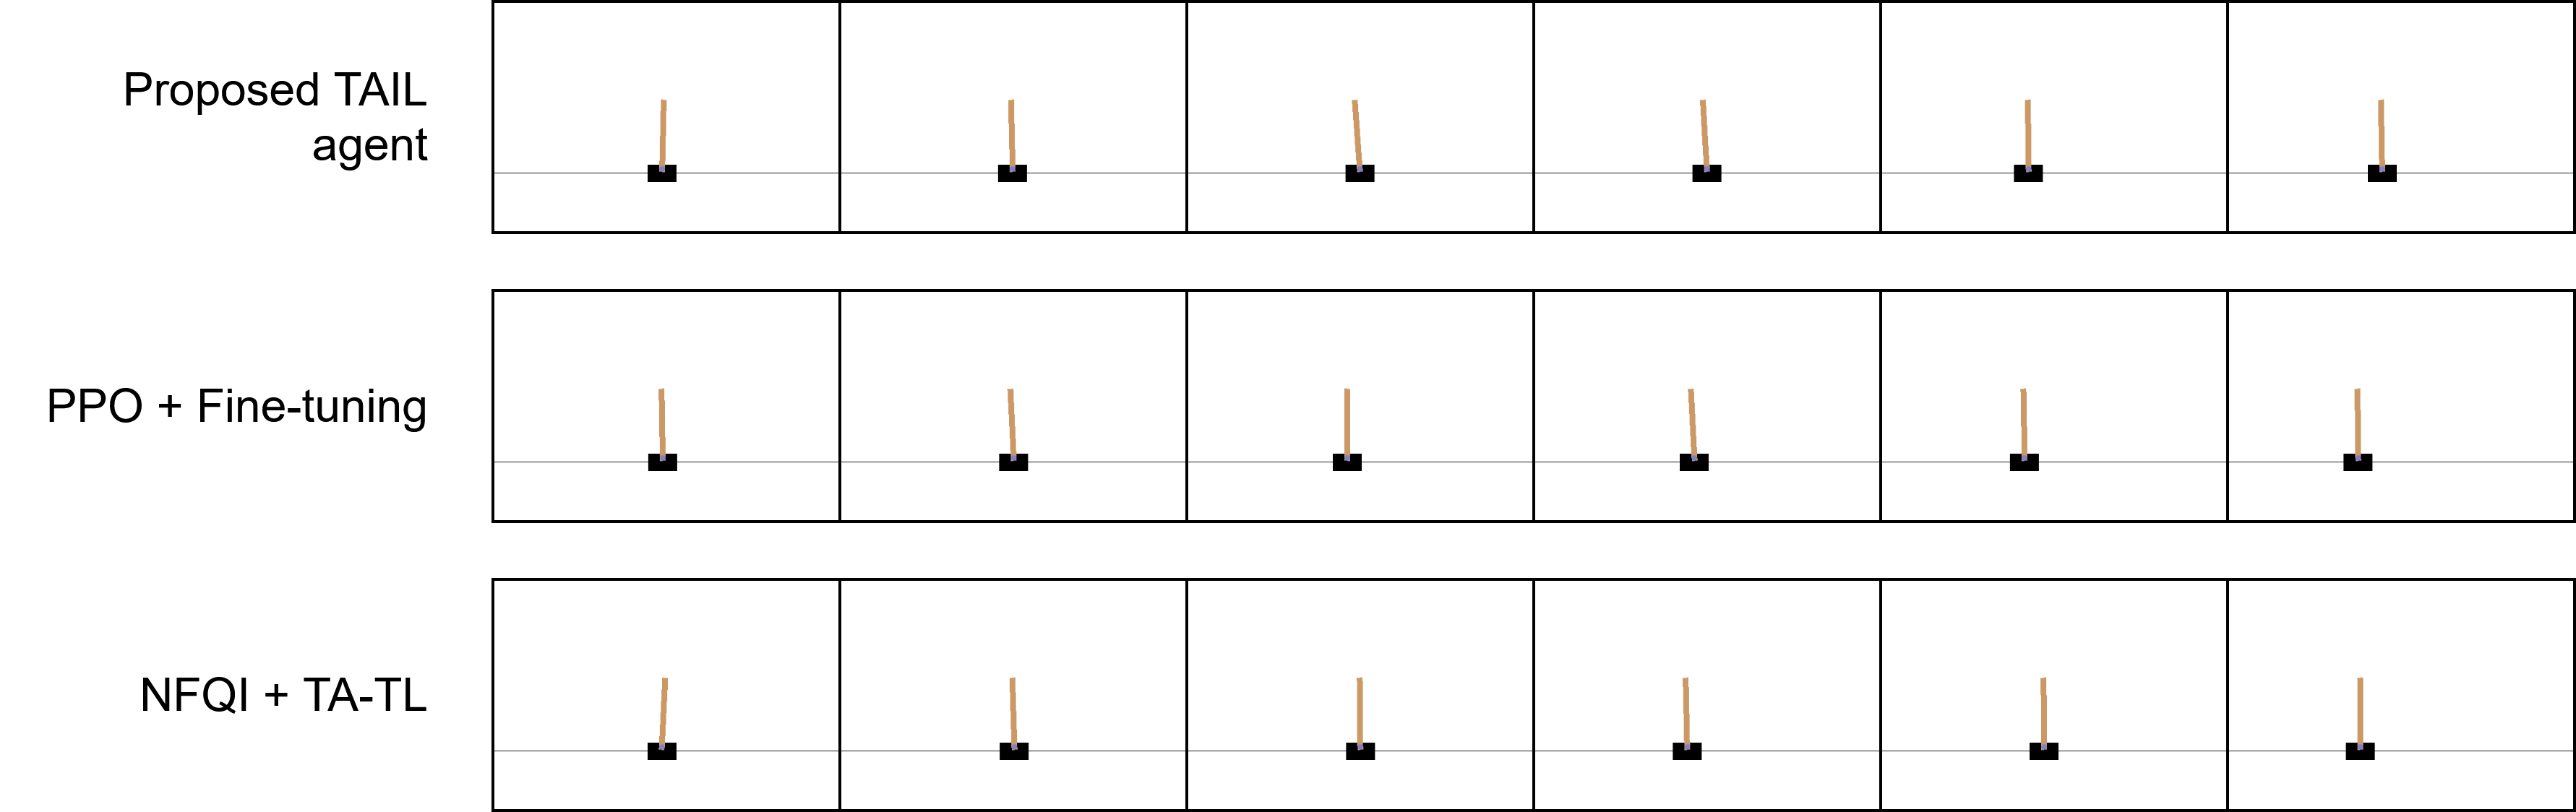
\includegraphics[width=\linewidth]{\FigsDir/Result_After_CartPole.png}
      \caption{\centering CartPole}
    \end{subfigure}
    %
    \par\bigskip
    %
    \begin{subfigure}[b]{\linewidth}
      \centering
      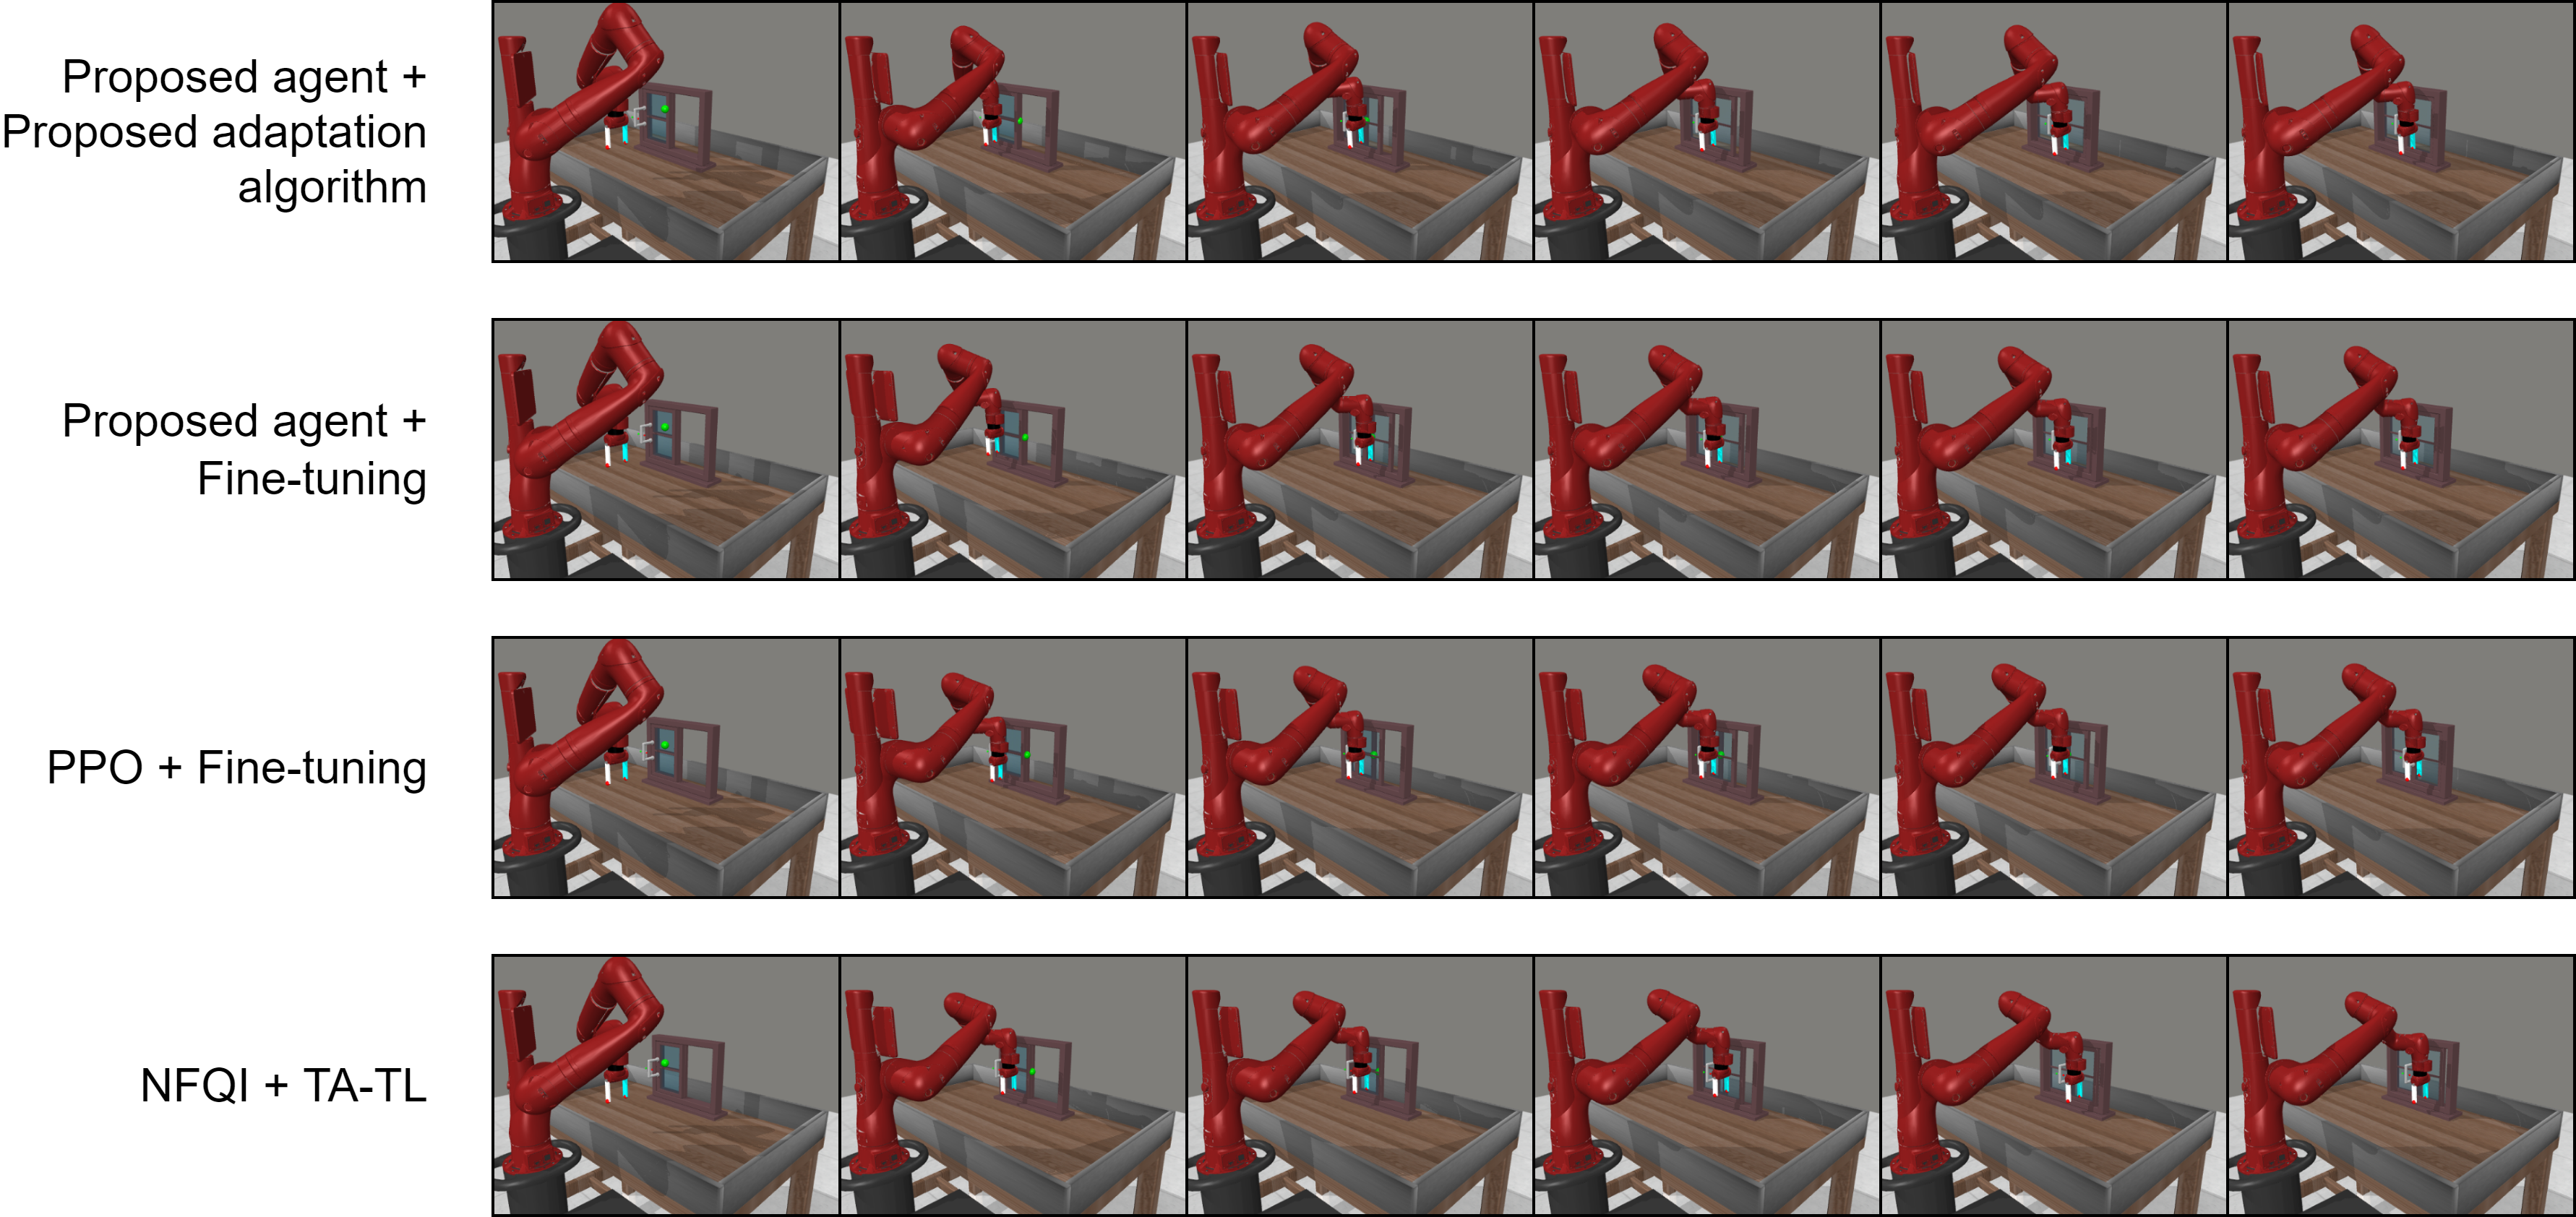
\includegraphics[width=\linewidth]{\FigsDir/Result_After_WindowClose.png}
      \caption{\centering WindowClose}
    \end{subfigure}
    %
    \caption{\textit{Cont}.}
  \end{figure}
  \begin{figure}[H]\ContinuedFloat
    \centering
    %
    \begin{subfigure}[b]{\linewidth}
      \centering
      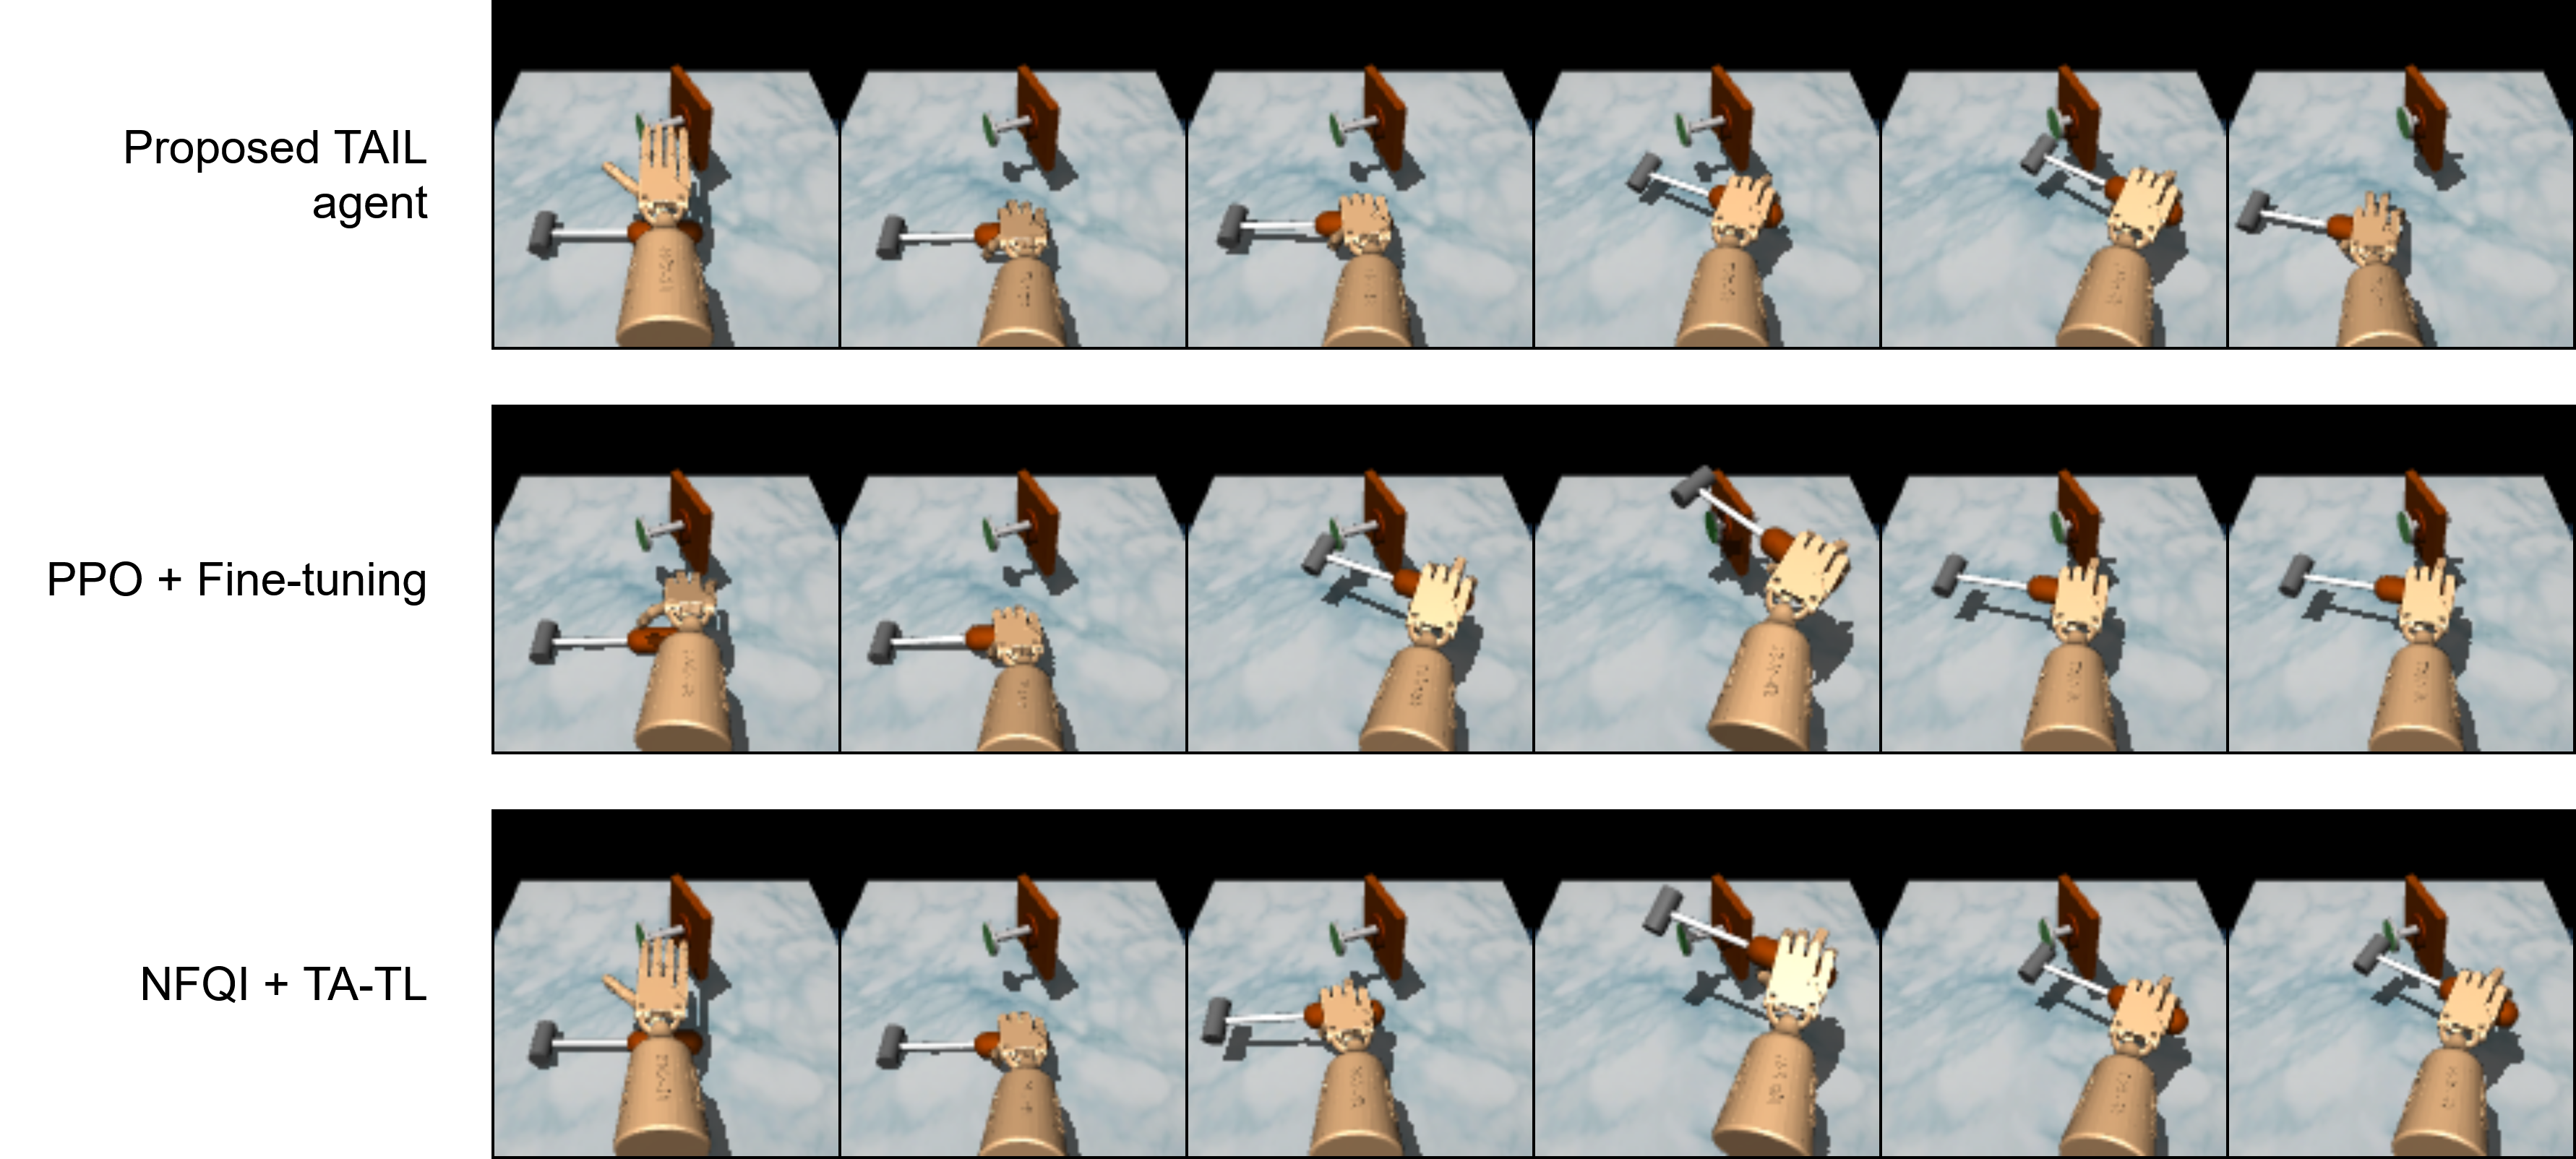
\includegraphics[width=\linewidth]{\FigsDir/Result_After_Hammer.png}
      \caption{\centering Hammer}
    \end{subfigure}
    %
    \caption{A visualization of the behavior of the proposed agent and baselines on target tasks.\label{fig:Result_After_Target}}
  \end{figure}
  \unskip
\end{landscape}

% \subsubsection{Computational Complexity}
% Besides evaluating the performance of the proposed agent in terms of success rate,
% its computational cost was also assessed in order to provide an adequate study of its overall performance.
% Table \ref{tab:Result_Cost} shows the training time required to train the agent in each experiment.
% It can be observed that the training time when applying fine tuning to PPO was slightly better than the training time of the proposed adaptation method,
% especially on two complex WindowOpen-WindowClose and Door--Hammer experiments.
% On the other hand, compared to TA-TL, the proposed adaptation method required a higher training time on all three experiments.
% This result was expected since,
% during the proposed adaptation process,
% the agent had to not only learn the new task, but also review the previously learned source task.
% However,
% it should be noted that the training time of the proposed adaptation method can be further improved by leveraging the parallel training process \cite{DL_Lib_StableBaselines3, DL_Lib_Tianshou}.


% \begin{table}[H]
%   \caption{The training time (s/epoch) of the proposed agent.\label{tab:Result_Cost}}

%   \centering
%   \begin{tabular}{lccc}
%     \toprule
%                                           & \textbf{Pendulum--CartPole} & \textbf{WindowOpen--WindowClose} & \textbf{Door--Hammer} \\
%     \midrule
%     \TAIL{}                               & 86.623                      & 165.768                          & 538.790               \\
%     PPO \cite{Baseline_PPO} + Fine-tuning & 84.234                      & 164.472                          & 534.234               \\
%     NFQI + TA-TL \cite{Baseline_TATL}     & 68.329                      & 129.420                          & 492.059               \\
%     \bottomrule
%   \end{tabular}
% \end{table}
